\subsection{Discussion}
First of all, it is important to state that we do not view measurement
clusterization as undesirable, nor do we believe it should be avoided
at all. Clusterization is a peculiar phenomenon and it is perfectly
reasonable for someone to argue against the D-optimality criterion
based on the fact that it results in clustered designs. We have seen,
however that there is perfectly reasonable explanation for
clusterization, i.e.~that clusterization arises when we seek a
designWe have shown that clusterization is an innevitable conseqeunce
of having a problem with modes of higher uncertainty than
others. Clusterization manifests the true underlying objective


\subsubsection{Answer to Question \ref{q:why}}
Theorem \ref{thm:char} helps us give a compelling explanation of the
measurement clusterization we obeserved for the inverse problem of the
heat equation (Fig.~\ref{fig:}). Below, we take the following steps:
We first utilize Theorem \ref{thm:char} to understand what a D-optimal
design will look like for our relaxed model; we then argue that
although not identical, a D-optimal design for the full inverse
problem of the heat equation shares similar charachteristics to the
relaxed design; finally, we show how ...

First, recall from Theorem \ref{thm:char} that in our relaxed model,
for a D-optimal design $\opt$:
\begin{enumerate}
  \item $\opt^*\opt$ is simultaneously diagonalizable with $\fwd
    \prcov \fwd^*$.
  \item $\opt^*\opt$ has non-zero eigenvalues only for the $k:=\rank
    \opt^*\opt$ smallest eigenvalues $\lambda_j$ of
    $\fwd\prcov\fwd^*$.
  \item $k$ is monotonic in $m$, the number of measurements we take.
\end{enumerate}

Now, consider $\fwd$ and $\prcov$ from the \emph{the inverse problem
of the heat equation}. As before, we denote the eigenvalues of
$\fwd\prcov\fwd^*$ by $\lambda_j$. We input these eigenvalues into our
\emph{relaxed} model, and find a D-optimal design $\opt$. In our
relaxed model, the measurements we take are best utilized in reducing
uncertainty for the first $k$ eigenvectors. So, a D-optimal design
arising from our \emph{relaxed model} completely avoids measuring
eigenvectors $k+1$ and above.

Of course, in a real life problem --- such as the inverse problem of
the heat equatiion --- it is likely impossible to find measurement
locations for which all eigenvectors $k+1$ and above are
zero. However, we can still expect a D-optimal design to give as
little weight as possible to eigenvectors $k+1$ and above. Thus a
D-optimal design is a trade-off between measuring eigenvectors we want
(eigenvectors for which $\lambda_j$ is large) and treating the rest as
noise.


We explore the abovementione trade-off for the inverse problem of the
heat equation in Fig.~\ref{fig:eigs}. We allow $m=4$ measurements in
$[0,1]$ and observe that D-optimal measurement locations are clustered
at $x_1 = 0.31$ and $x_2 = 0.69$. Upon close inspection of the scaled
eigenvectors of $\fwd \prcov \fwd^*$, we first observe that
eigenvectors $3$ and above have negligible prior amplitude. Since we
only have $m=4$ measurements at our disposal, Theorem \ref{thm:char}
tells us we should only care about measuring the first and second
eigenvectors. Then, we note the D-optimal $x_1,x_2$ present a
compromise between the amplitude of the first and second
eigenvectors. For example, a measurement at $x=0.5$ would have ignored
the second eigenvector altogether, since its value is zero at $x=0.5$.
Now we can understand measurement clusterization: attempting to
measure what we want and ignoring the rest, along with the spatial
limitations on measurements imposed by the structure of eigenvectors
of $\fwd \prcov \fwd^*$ is the cause for measurement clusterization in
D-optimal designs.


%% In the inverse problem of the heat equation, \ev_3, \ev_4,\dots$
%% implies we seek measurement locations for which $\lambda_1\ev_1,
%% \lambda_2\ev_2$ are large, while $\lambda_3\ev_3,
%% \lambda_3\ev_3,\dots$ are small. It turns out that there are two
%% locations that give the best trade-off, and measurements are taken in
%% those two locations. Once we have more than two measurements at our
%% disposal, measurement locations becomde clustered, by the pigeonhole
%% principle, see Fig.~\ref{fig:eigenvectors}.

%% The way a D-optimal design tries to ignore all eigenvectors
%% corresponding to $j > 2$. Since $\lambda_j$ decay to zero, a D-optimal
%% design should only try to avoid eigenvectors for which $\lambda_j$ is
%% not already small --- e.g.~eigenvectors $j=3,4$. It is possible that
%% the geometry of the domain $\Omega$ and the structure of the
%% eigenvectors leave only a few locations in $\Omega$ where the
%% amplitude of eigenvectors $j=1,2$ is high while the amplitude of
%% eigenvectors $j=3,4$ is low. In such case, clusterization will occur
%% whenever the number of measurements $m$ is large enough, by the
%% pigeonhole principle. This scenario is illustrated for the inverse
%% problem of the 1D heat equation in Fig.~\ref{fig:eigenvectors}.

\begin{figure}\label{fig:eigenvectors}
    \centering
    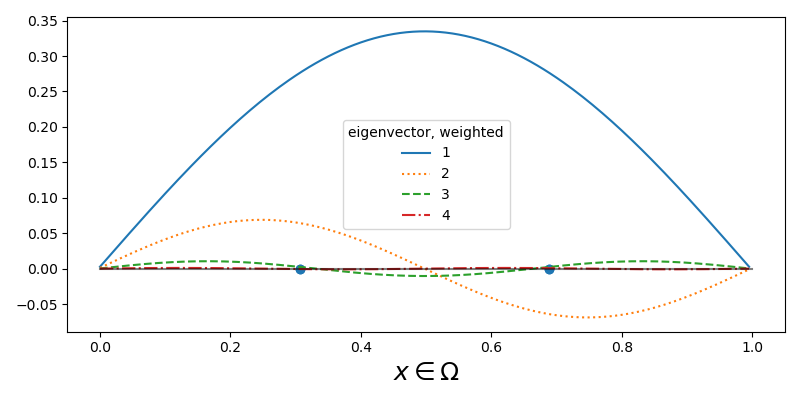
\includegraphics[width=\textwidth]{eigenvectors_dst_scaled.png}
    \caption{D-optimal measurement locations ($m=4$ measurements) and
      weighted eigenvectors for finding the initial condition of
      the 1D heat equation. Measurement locations and weighted
      eigenvectors are plotted over the computational domain $\Omega =
      [0, 1]$ (x-axis). Measurement clusterization occurs
      approximately at $0.31$ and $0.69$. These two locations are a
      compromise between zeros of eigenvectors a D-optimal design aims
      to ignore (third and up) and staying far from zeros of the
      eigenvectors a D-optimal design aims to measure (first and
      second). Allocating $m=4$ measurements into two locations
      results in clusterization, according to the pigeonhole
      principle.}
  \label{fig:why}
\end{figure}


As mentioned in the Limitations section, our model does not accomodate
point evaluations. For example, in the inverse problem of the 1D heat
equation, it seems reasonable to take $\hilp = \hilo =
L^2(\Omega)$. Unfortunately, for any point evaluation $\delta_x \not
\in L^2(\Omega)$.are taken of the final heat distribution $u_T$. If we
consider the initial and final conditions $u_0$ and $u_T$ as elements
of $L^2([0,1])$, theheat equation as
